%----------------------------------------------------------------------------------------
%	PACKAGES AND OTHER DOCUMENT CONFIGURATIONS
%----------------------------------------------------------------------------------------

\documentclass[paper=a4, fontsize=11pt]{scrartcl} % A4 paper and 11pt font size

\usepackage[margin=1.0in]{geometry}	%for some reason, looks beter. 

\usepackage[T1]{fontenc} % Use 8-bit encoding that has 256 glyphs
\usepackage{fourier} % Use the Adobe Utopia font for the document - comment this line to return to the LaTeX default
\usepackage[english]{babel} % English language/hyphenation
\usepackage{amsmath,amsfonts,amsthm} % Math packages

\usepackage{lipsum} % Used for inserting dummy 'Lorem ipsum' text into the template

\usepackage{sectsty} % Allows customizing section commands
\allsectionsfont{\centering \normalfont\scshape} % Make all sections centered, the default font and small caps

\usepackage{fancyhdr} % Custom headers and footers
\pagestyle{fancyplain} % Makes all pages in the document conform to the custom headers and footers
\fancyhead{} % No page header - if you want one, create it in the same way as the footers below
\fancyfoot[L]{} % Empty left footer
\fancyfoot[C]{} % Empty center footer
\fancyfoot[R]{\thepage} % Page numbering for right footer
\renewcommand{\headrulewidth}{0pt} % Remove header underlines
\renewcommand{\footrulewidth}{0pt} % Remove footer underlines
\setlength{\headheight}{13.6pt} % Customize the height of the header

\numberwithin{equation}{section} % Number equations within sections (i.e. 1.1, 1.2, 2.1, 2.2 instead of 1, 2, 3, 4)
\numberwithin{figure}{section} % Number figures within sections (i.e. 1.1, 1.2, 2.1, 2.2 instead of 1, 2, 3, 4)
\numberwithin{table}{section} % Number tables within sections (i.e. 1.1, 1.2, 2.1, 2.2 instead of 1, 2, 3, 4)

\setlength\parindent{0pt} % Removes all indentation from paragraphs - comment this line for an assignment with lots of text

%----------------------------------------------------------------------------------------
%Personal Packages and File Dependencies 
%----------------------------------------------------------------------------------------	

\usepackage{graphicx}	%insert graphics
\usepackage{microtype}	%improves spacing
\usepackage{float}		%H postion	
\usepackage{caption}	%caption w/o : 	
\usepackage{framed}		%creates frames
\usepackage{enumitem}
\usepackage{nag}

\usepackage{listings}	%insert sourcecode
\usepackage{color}
\usepackage{pdfpages}	%include PDF pages

\usepackage{bigstrut}	%exce2latex table packages
\usepackage{rotating}
\usepackage{multirow}
\usepackage{booktabs}
%\usepackage[framed]{mcode}

\usepackage{cleveref}	%cooler references, needs to be last
\usepackage[bookmarks]{hyperref}
\graphicspath{{../Figures/}{../figures/}} % This automatically connects to the figure folder

%----------------------------------------------------------------------------------------
%	TITLE SECTION
%----------------------------------------------------------------------------------------

\newcommand{\horrule}[1]{\rule{\linewidth}{#1}} % Create horizontal rule command with 1 argument of height

\title{	
\normalfont \normalsize 
\textsc{TEMPLE UNIVERSITY COLLEGE OF ENGINEERING | ECE 3623 | SPRING 2015} \\ [25pt] % Your university, school and/or department name(s)
\horrule{0.5pt} \\[0.4cm] % Thin top horizontal rule
\huge Computer Assignment (CA) No. 8: 
Central Limit Theorem \\ % The assignment title
\horrule{2pt} \\[0.5cm] % Thick bottom horizontal rule
}

\author{Tyler Berezowsky} % Your name

\date{\normalsize\today} % Today's date or a custom date 
\usepackage{mcode}

\begin{document}
\maketitle % Print the title

\section{Problem Statement} 
%Summarize the problem statement in one paragraph. Clearly state what the knowns are and what unknowns you must find.
The purpose of this assignment was to explore methods to calculate  variance in real time, and create a distinction between those methods. Comparison was also made to the global variance. This was accomplished through MATLAB, the previously used data sets and the following tasks: 
\begin{enumerate}
\item Estimate the variance (second central moment) from the entire data set. Plot this as a horizontal dotted line.
\item Starting with the first 10 samples, estimate the variance from the first N samples of the signal, letting N vary from 0 to a maximum of the number of samples in the file. Overlay a plot of this on the plot from (1). Describe what you observe.
\item Now estimate the variance using a frame/window approach. For the Google stock price, set the frame to 1 day and the window to 30 days. For the speech signal, set the frame duration to 10 msec and the window duration to 30 msec. Overlay this plot on the above plot and describe what you observe. Which approach makes sense?
\end{enumerate}

\section{Approach and Results} 
%Describe your approach to finding the unknowns. Use numbered figures, tables and equations where necessary.
The data sets were loaded via code from previous computer assignments. For task one, the global variance was determined through the \verb|var()| command. For task two, the rolling calculation was performed through a \verb|for loop| which selected a subset of data always starting at the origin. The subset was increased by 10 samples per iteration until the subset was the length of the original set. At each iteration, the variance of the subset was calculated (via \verb|var()|) developing a rolling calculation of variance for the data set. For task two, frame and windowing was accomplished through code from CA: 01. Variance was calculated for the audio signal with a frame size of 10 msec and a window size of 30msec.  Variance of the google data set was calculated with a frame size of 1 day and a window size of 30 days. \\ 

For each respective data set, the global, rolling, and framed variance was plotted together. The plots can be seen in figures~\ref{fig: audio} and \ref{fig: google}. The trace legend for both plots is identical. The blue trace represents the rolling variance, the red trace represents the framed variance, and the orange trace represents the global variance. 

\begin{figure}[H] 
	\centering 
	\includegraphics[width=\linewidth]{plot_01_1}
	\caption{Plot of global, rolling, and framed and windowed variance overlaid for the audio signal.}
	\label{fig: audio} 
\end{figure}


Interesting to note for the audio plot, is the self leveling behavior of the rolling variance  with the global variance. When the subset is small, at the beginning of the signal, ripples of a diminishing nature can be observed. This of course correlates to the spikes of variance or energy (due to a near zero mean) present in the audio signal. The energy spikes, relatively constant in amplitude and period, between 0 and 3 seconds begin to level the rolling variance as the carnality of the sample set increases until the large energy spike between 3 and 4 seconds upsets the rolling variance. As the carnality of the sample set increases again with  energy spikes of a more uniform amplitude, but less than then those near the origin of the signal, the rolling variance begins to diminish and level again with the global mean between the 4 and 10 second mark. \\

The rolling calculation is self leveling with the global variance because it is constantly approaching it with each increase of the subset. As the subset increases, the spikes in variation also become more illusive. This behavior can be illustrated through the variance calculation: 
\begin{equation}
\sigma^2 = \frac{1}{N}\sum_{i=1}^{n}(x_i - \bar{x})^2
\end{equation}
As the set increases, the large number of relatively constant sums and increasing denominator N, level any variation in variance. This effect is directly correlated to the size of the set. Therefore, a rolling variance calculation would not be effective at determining local variation in signal amplitude. Frame and windowing is a more suitable technique as it permits sections of the signal to be examined which then can be compared to the global variance or rolling variance for real time applications.  

 \begin{figure}[h] 
 	\centering 
 	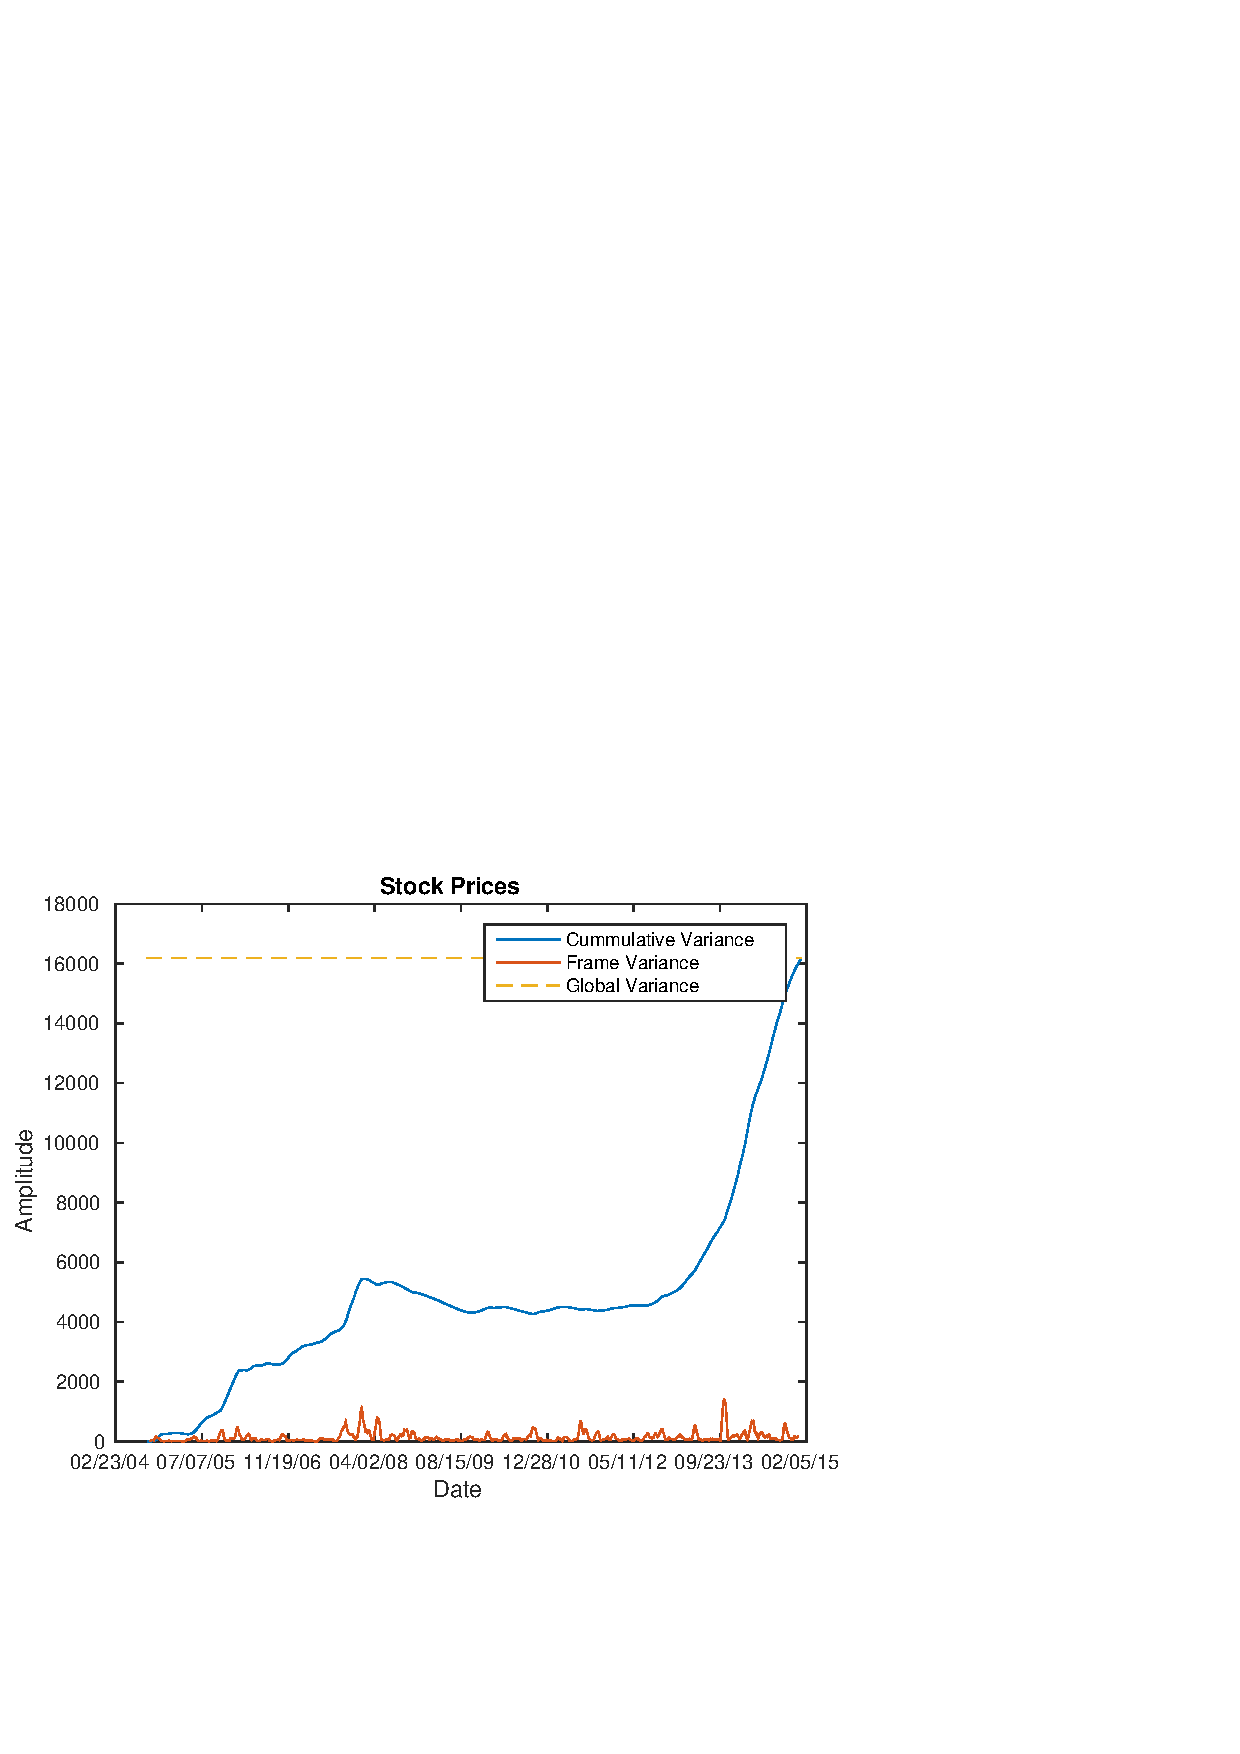
\includegraphics[width=\linewidth]{plot_02_1}
 	\caption{Plot of global, rolling, and framed and windowed variance overlaid for the Google stock.}
 	\label{fig: google} 
 \end{figure}
 
 The Google stock plot illustrates an increasing rolling variance which ends at the global variance, with minimal deviation in variance per frame compared to the audio signal. 
 This is distinct in comparison to the audio signal's rolling variance which tracked the global variance. This behavior is due to the completely random nature of the samples and positive non-irregular trend in the stock data set. \\
 
 In layman's terms, the samples can be seen to be regularly increasing, and therefore generally never identical. In perspective of the variance calculation, a data set with a positive trend will be constantly increasing in variation as each sample is different from the last. This is also true for a signal with a negative trend. A flat lined signal would produce no variation as the mean would always cancel the numerator. And as with the audio signal, a signal with samples that illustrate a high degree of variance in a predicable manner, will illustrate a uniform amount of variance.   
 
 
\section{MATLAB Code} 
%Show and briefly explain your MATLAB code.
\lstinputlisting[frame=single,caption=MATLAB solution for CA: 03, label=MATLAB]{../MATLAB/ca_03.m}

\section{Conclusions} 
%Summarize what you found.
This assignment illustrated two methods of calculating variance in ``real-time'': rolling and framed. Comparison was also made to global variance for each method. \\

The following conclusions were made. First, rolling variance calculations are not effective for determining local changes in variance. As the size of a sample set increases, small bursts of variance will become washed out due to averaging effect of the large set. Frame and windowing the data set, and then calculating the variance of the window is a more sensitive approach. Secondly, a digital audio signal contains a finite amount of possible values. Therefore, it is possible to predict the probability of the next sample which is ironic (to me atleast) as it contains no discernible trend besides averaging to zero. Last, and even weirder, while the Google stock data contains a trend, it is completely unpredictable through a classic probability spaces (As far as I currently know!?) as the $\Omega$ set increases with each sample. This is illustrated in the accumulating rolling variance due to the positive trend in the Google stock price present in figure~\ref{fig: google}. 

\end{document}